\documentclass[main.tex]{subfiles}
\begin{document}\newpage
\setdoublesep{0.35700 em}  % 'Bond Spacing'
\setatomsep{1.78500 em}    % 'Fixed Length'
\setbondoffset{0.18265 em} % 'Margin Width'
\newcommand{\bondwidth}{0.06642 em} % 'Line Width'
\setbondstyle{line width = \bondwidth}

\begin{fullwidth}





%%%%%%%%%%%%HEADING
\begin{multicols}{2}
\begin{tcolorbox}[enhanced jigsaw,breakable,size=title,
colback=mybrown!05,colframe=black,fonttitle=\bfseries,
title=STUDENT INFO,pad at break=1mm, break at=15cm/0pt ]
\vspace{0.2cm}
\noindent Name: \rule{5cm}{0.4pt}Date:\rule{1cm}{0.4pt}\\
Pre-lab Done: \tikzcheckmark[scale=2,black]{no mark}\quad
\end{tcolorbox}
\end{multicols}
\hfill
\vspace{0.2cm}
\begin{center}
{\large \bfseries 
Pre-lab Questions 
\par
\Huge
Density
\\[5pt] \par}
\vspace{0.2cm}
\end{center}
\par
\noindent
\uline{  \hfill \normalsize \hfill       }
%%%%%%%%%%%%HEADING

\begin{enumerate}
% PELAB 1
\item Do oil float on water? Explain why.
\vspace{3cm}

\item Research the meaning of specific gravity.
\vspace{3cm}

\item A 3g glucose solution occupies a volume of 0.1L. Calculate the density of the solution in g/mL.
\vspace{3cm}


\item Oil has a density of 0.9g/mL.  Calculate the mass of a 100mL oil sample.
\vspace{3cm}


\item An electrolyte solution has a density of 1.3g/mL.  Calculate the volume in L of a 2mg  sample.
\vspace{3cm}



\end{enumerate}


\clearpage\mbox{}\clearpage



%%%%%%%%%%%%HEADING
\begin{multicols}{2}
\begin{tcolorbox}[enhanced jigsaw,breakable,size=title,
colback=mybrown!05,colframe=black,fonttitle=\bfseries,
title=STUDENT INFO,pad at break=1mm, break at=15cm/0pt ]
\vspace{0.2cm}
\noindent Name: \rule{5cm}{0.4pt}Date:\rule{1cm}{0.4pt}\\
Pre-lab Done: \tikzcheckmark[scale=2,black]{no mark}\quad
\end{tcolorbox}
\end{multicols}
\hfill
\vspace{0.2cm}
\begin{center}
{\large \bfseries 
Experiment
\par
\Huge
Density
\\[5pt] \par}
\vspace{0.2cm}
\end{center}
\par
\noindent
\uline{  \hfill \normalsize \hfill       }
%%%%%%%%%%%%HEADING

\vspace{0.2cm}{\large \bfseries 1. Density of water}
The goal of this mini-experiment is to calculate the density of water. In order to do this you will measure the mass of a specific volume of water and use the formula for density:
\begin{equation*}
d=\frac{m}{V}
\end{equation*}
\begin{steps}
    \newstep[] Place approximately 25mL of tab water into a 100mL cylinder. Indicate the exact volume you employed in the table below.    
    \newstep[] Place a 100mL (or 25mL) beaker in the scale and press zero. After that add the liquid from the cylinder and write down the mass in the table below.
     \newstep[] Compute the value of density.
\end{steps}

\begin{center}\begin{tabular}{ |p{4cm}|p{4cm}|p{4cm}|  }
\hline
    Volume (mL) &  mass (g) &  Density  (g/mL)         \\
\hline
   \vspace{0cm}\vspace{.5cm} &     &            \\
\hline
\end{tabular}\end{center}


\vspace{0.2cm}{\large \bfseries 2. Density of a solution}
In this section you will calculate the density of an unknown solution by repeating the procedure from the previous mini-experiment. You will also compute the specific gravity by diving the density of the solution by the density of water.
\begin{equation*}
\text{specific gravity}=\frac{d}{d_{water}}
\end{equation*}

\begin{steps}
    \newstep[] Place approximately 25mL of the solution into a 100mL cylinder. Indicate the exact volume you employed in the table below.    
    \newstep[] Place a 100mL (or 25mL) beaker in the scale and press zero. After that add the liquid from the cylinder and write down the mass in the table below.
     \newstep[] Compute the value of density.
\end{steps}
\begin{center}\begin{tabular}{ |p{4cm}|p{4cm}|p{4cm}|  }
\hline
    Volume (mL) &  mass (g) &  Density  (g/mL)         \\
\hline
   \vspace{0cm}\vspace{.5cm} &     &            \\
\hline
    Density  solution (g/mL)  &  Density  water (g/mL) &  Specific Gravity      \\
\hline
   \vspace{0cm}\vspace{.5cm} &     &            \\
\hline
\end{tabular}\end{center}

\end{fullwidth}




\newpage
\begin{fullwidth}
\vspace{0.2cm}{\large \bfseries 3. Density of a solid}
In this mini-experiment you will calculate the density of a metal by a method called volume displacement. You will measure the volume of a liquid before and after adding the solid The difference in volume is the volume of the solid. By means of this measurement and the mass of the solid you will be able to estimate density. 
\begin{steps}
    \newstep[] Obtain a metallic object and weight it. Record its mass in the table below.
        \newstep[]  Attach a string to the object and submerge it in a 50mL cylinder big enough to fit the object. 
        \newstep[]  Add water until the object is covered. Record this volume in the table below.   
         \newstep[] Now using the string remove the object from the cylinder. Write down the liquid volume after the object is out.
      \newstep[] Calculate the volume of the object by subtracting the liquid volume before and after removing the object from the cylinder.
       \newstep[] Use the formula of density to calculate the density of the solid.     
\end{steps}

\begin{center}\begin{tabular}{ |p{2cm}|p{3.5cm}|p{5.5cm}|p{3.5cm}|p{2.5cm}|  }
\hline
    Mass (g) &  Volume before adding the object (mL) & Volume after adding he object (mL)& V(After)-V(Before) (mL)& Density (g/mL)         \\
\hline
   \vspace{0cm}\vspace{.5cm} &     &   &&         \\
\hline
\end{tabular}\end{center}


\vspace{0.2cm}{\large \bfseries 5. Density by graphing }
The goal of this mini-experiment is to calculate the density of a metal by means of a graph. This method is useful for small pieces of metal which volume can not be computed by means of the volume displacement method. You will continuously add pieces of metal to a liquid so that the volume will progressively increase.  By graphing mass vs. volume you will be able to compute density.
\begin{steps}
        \newstep[]  Place 25mL of water in a 100mL cylinder. Carefully record the liquid volume in the table below.
    \newstep[] By means of a scale calculate the volume of the liquid and record the value      
    \newstep[] Add metal pieces (or perhaps pennies) so that the liquid volume changes significantly. Write down the new volume and the new mas.
            \newstep[] Keep on adding metal pieces until you fill in the table below.
               \newstep[] Plot mass (vertical axis) vs. volume (horizontal axis) in the graph below.
  \newstep[] You will calculate the density of the metal by selecting two arbitrary points from the plot (point 1 and point 2, where point 2 has a larger mass) and using the formula:
\begin{equation*}
\text{density}=\frac{mass(2)-mass(1)}{volume(2)-volume(1)}=\frac{\hspace{5cm}}{}=\hspace{3cm} g/mL
\end{equation*}
\end{steps}

\begin{center}\begin{tabular}{ |p{3cm}|p{5cm}| }
\hline
    Volume (mL) &  mass (g)        \\
\hline
   \vspace{0cm}\vspace{.5cm} &           \\
\hline
   \vspace{0cm}\vspace{.5cm} &                 \\
\hline
   \vspace{0cm}\vspace{.5cm} &                 \\
\hline
   \vspace{0cm}\vspace{.5cm} &                 \\
\hline
   \vspace{0cm}\vspace{.5cm} &                 \\
\hline
  \vspace{0cm}\vspace{.5cm} &                 \\
\hline
  \vspace{0cm}\vspace{.5cm} &                 \\
\hline
  \vspace{0cm}\vspace{.5cm} &                 \\
\hline
  \vspace{0cm}\vspace{.5cm} &                 \\
\hline
\end{tabular}\end{center}



\end{fullwidth}


\newpage
\begin{fullwidth}
\begin{center}
 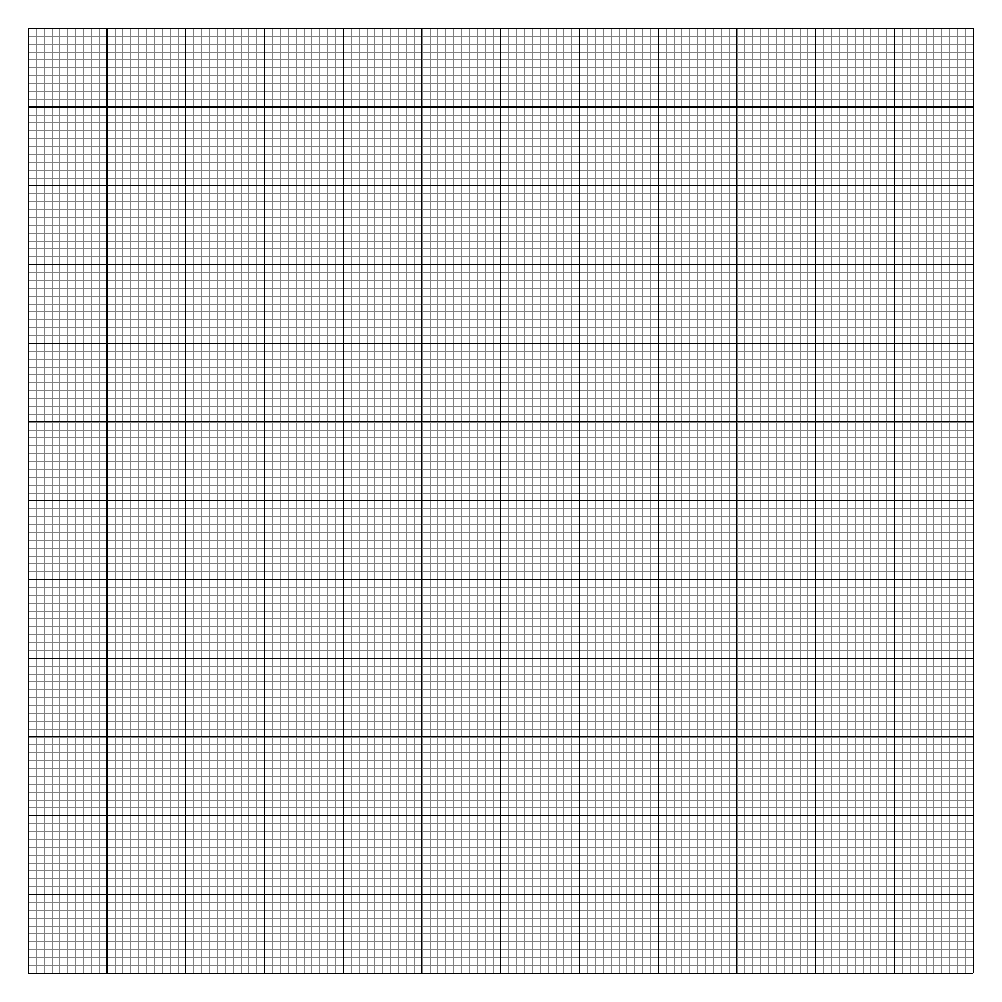
\begin{tikzpicture}
 \draw[step=1mm,help lines] (0,0) grid (120mm,120mm);
 \draw[step=10mm] (0,0) grid (120mm,120mm);
\end{tikzpicture}\\
\vspace{0.2cm}
Name of metal=\rule{5cm}{0.4pt}
\end{center}

\vspace{0.2cm}{\large \bfseries 6. PostLab questions }

\begin{enumerate}
\item 
A nugget of metal with a mass of 400 g is added to 25.0 mL of water.  The water level rises to a volume of 40 mL.  What is the density of the metal?   

\vspace{2.5cm}
\item Determine the density (g/mL) of a 0.3 L sample of a salt solution that has a mass of 40 g.
\vspace{2.5cm}

\item A graduated cylinder contains 25 mL of water. What is the new water level after
35 g of silver metal is submerged in the water if the density of silver is 11g/mL?\vspace{2.5cm}

\end{enumerate}



\end{fullwidth}



\end{document}